
\documentclass{beamer}
\usecolortheme{dove}
\setbeamertemplate{navigation symbols}{}
\usepackage{amsmath,amssymb,amsfonts,amsthm, multicol, subfigure, color}
\usepackage{bm}
\usepackage{graphicx}
\usepackage{tabularx}
\usepackage{booktabs}
\usepackage{hyperref}
\usepackage{pdfpages}
\usepackage{xcolor}
\definecolor{seagreen}{RGB}{46, 139, 87}
\definecolor{mustard}{RGB}{234, 170, 0}
\def\independenT#1#2{\mathrel{\rlap{$#1#2$}\mkern2mu{#1#2}}}
\newcommand\indep{\protect\mathpalette{\protect\independenT}{\perp}}
\def\log{\text{log}}
\newcommand\logit{\text{logit}}
\newcommand\iid{\stackrel{\text{iid}}{\sim}}
\newcommand\E{\text{E}}
\newcommand\V{\text{V}}
\renewcommand\P{\text{P}}
\newcommand{\Cov}{\text{Cov}}
\newcommand{\Cor}{\text{Cor}}
\newcommand\doop{\texttt{do}}
\usepackage{stackrel}
\usepackage{tikz}
\usetikzlibrary{arrows,shapes.arrows,positioning,shapes,patterns,calc}
\newcommand\slideref[1]{\vskip .1cm \tiny \textcolor{gray}{{#1}}}
\newcommand\red[1]{\color{red}#1}
\newcommand\blue[1]{\color{blue}#1}
\newcommand\gray[1]{\color{gray}#1}
\newcommand\seagreen[1]{\color{seagreen}#1}
\newcommand\purple[1]{\color{purple}#1}
\newcommand\orange[1]{\color{orange}#1}
\newcommand\black[1]{\color{black}#1}
\newcommand\white[1]{\color{white}#1}
\newcommand\teal[1]{\color{teal}#1}
\newcommand\magenta[1]{\color{magenta}#1}
\newcommand\Fuchsia[1]{\color{Fuchsia}#1}
\newcommand\BlueGreen[1]{\color{BlueGreen}#1}
\newcommand\bblue[1]{\textcolor{blue}{\textbf{#1}}}
\newcommand\bred[1]{\textcolor{red}{\textbf{#1}}}
\newcommand\bgray[1]{\textcolor{gray}{\textbf{#1}}}
\newcommand\bgreen[1]{\textcolor{seagreen}{\textbf{#1}}}
\newcommand\bref[2]{\href{#1}{\color{blue}{#2}}}
\colorlet{lightgray}{gray!40}
\pgfdeclarelayer{bg}    % declare background layer for tikz
\pgfsetlayers{bg,main} % order layers for tikz
\newcommand\mycite[1]{\begin{scriptsize}\textcolor{darkgray}{(#1)}\end{scriptsize}}
\newcommand{\tcframe}{\frame{
%\small{
\only<1|handout:0>{\tableofcontents}
\only<2|handout:1>{\tableofcontents[currentsubsection]}}
%}
}

\newcommand{\goalsframe}{\begin{frame}{Learning goals for today}
By the end of class, you will be able to
\begin{itemize}
    \item argue about economic mobility as a measure of opportunity
    \item frame economic mobility as a prediction question
\end{itemize} \vskip .2in
\end{frame}}

\usepackage[round]{natbib}
\bibliographystyle{humannat-mod}
\setbeamertemplate{enumerate items}[default]
\usepackage{mathtools}

\title{Studying Social Inequality with Data Science}
\author{Ian Lundberg}
\date{\today}

\begin{document}

\begin{frame}
\begin{tikzpicture}[x = \textwidth, y = \textheight]
\node at (0,0) {};
\node at (1,1) {};
\node[anchor = north west, align = left, font = \huge] at (0,.9) {Studying\\Social Inequality\\with Data Science};
\node[anchor = north east, align = right] (number) at (1,.9) {INFO 3370 / 5371\\Spring 2023};
\node[anchor = north, font = \Large, align = right] at (.5,.5) {\bblue{Opportunity}\\As measured by economic mobility};
\end{tikzpicture}
\end{frame}

\goalsframe

\begin{frame}
Before class, you read the intro and discussion of:
\begin{itemize}
\item Chetty et al. 2014. \bref{https://eml.berkeley.edu/~saez/chettyetalAERPP2014.pdf}{Is the United States Still a Land of Opportunity? Recent Trends in Intergenerational Mobility}. American Economic Review 104(5):141--147. 
\end{itemize} \vskip .3in
Let's discuss
\begin{itemize}
\item The ladder metaphor
\item Changes in inequality
\item Changes in rank-based mobility
\end{itemize} \vskip .15in
Then we will look at figures
\end{frame}

\begin{frame}
\includegraphics[width = \textwidth]{figures/chetty_fig1}
\end{frame}

\begin{frame}
\includegraphics[width = \textwidth]{figures/chetty_fig3}
\end{frame}

\begin{frame}
Additional evidence from a paper you did not read:
\begin{itemize}
\item Chetty et al. 2017. \bref{https://www.science.org/doi/full/10.1126/science.aal4617}{The fading American dream: Trends in absolute income mobility since 1940.} Science 356.6336:398-406.
\end{itemize}
This paper
\begin{itemize}
\item assumes that rank-based mobility was constant
\item given that assumption, focuses on \bgray{absolute} mobility
\end{itemize}
\end{frame}

\begin{frame}
\includegraphics[width = \textwidth]{figures/chetty2017_fig1b}
\end{frame}

\begin{frame}
\includegraphics[width = \textwidth]{figures/chetty2017_fig2b}
\end{frame}

\begin{frame}
\includegraphics[width = \textwidth]{figures/chetty2017_fig2c}
\end{frame}

\begin{frame}
The probability that a child out-earns their parent has fallen
\end{frame}

\begin{frame}{Generalizing these ideas}

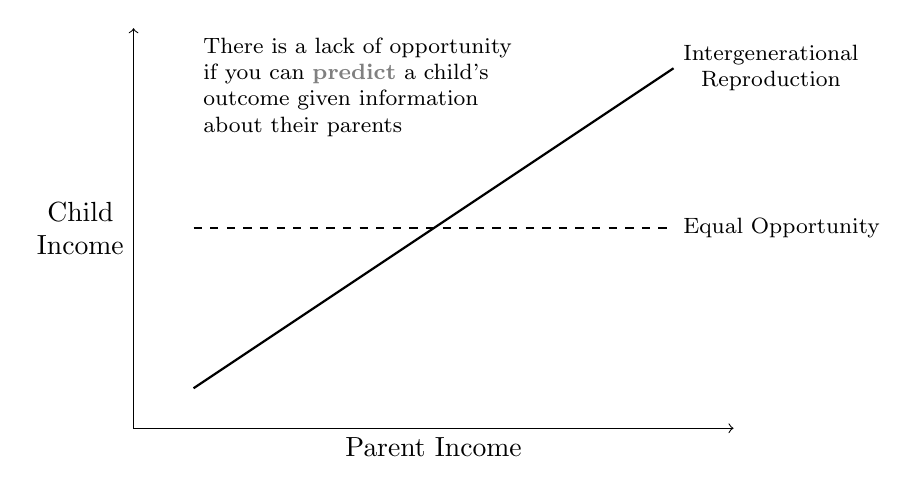
\begin{tikzpicture}[x = 3in, y = 2in]
\draw[<->] (1,0) -- (0,0) -- (0,1);
\node[anchor = east, align = center] at (0,.5) {Child\\Income};
\node[anchor = north, align = center] at (.5,0) {Parent Income}; \pause
\draw[thick, dashed] (.1,.5) -- (.9,.5);
\node[anchor = west, font = \footnotesize] at (.9,.5) {Equal Opportunity}; \pause
\draw[thick] (.1,.1) -- (.9,.9);
\node[anchor = west, font = \footnotesize, align = center] at (.9,.9) {Intergenerational\\Reproduction}; \pause
\node[anchor = north west, font = \footnotesize, align = left] at (.1,1) {There is a lack of opportunity\\if you can \bgray{predict} a child's\\outcome given information\\about their parents};
\end{tikzpicture}

\end{frame}

\goalsframe

\end{document}

